\section{PSR J0737$-$3039A: Characterizing a Double Pulsar System with Finite-Altitude Model}
\paperref{This section is based on work done for ``\it{Fermi} LAT Pulsed
Detection of PSR J0737$-$3039A in the Double Pulsar System'' \citep{guillemot2013fermi}.}

\begin{figure*}[t!!]
\begin{center}
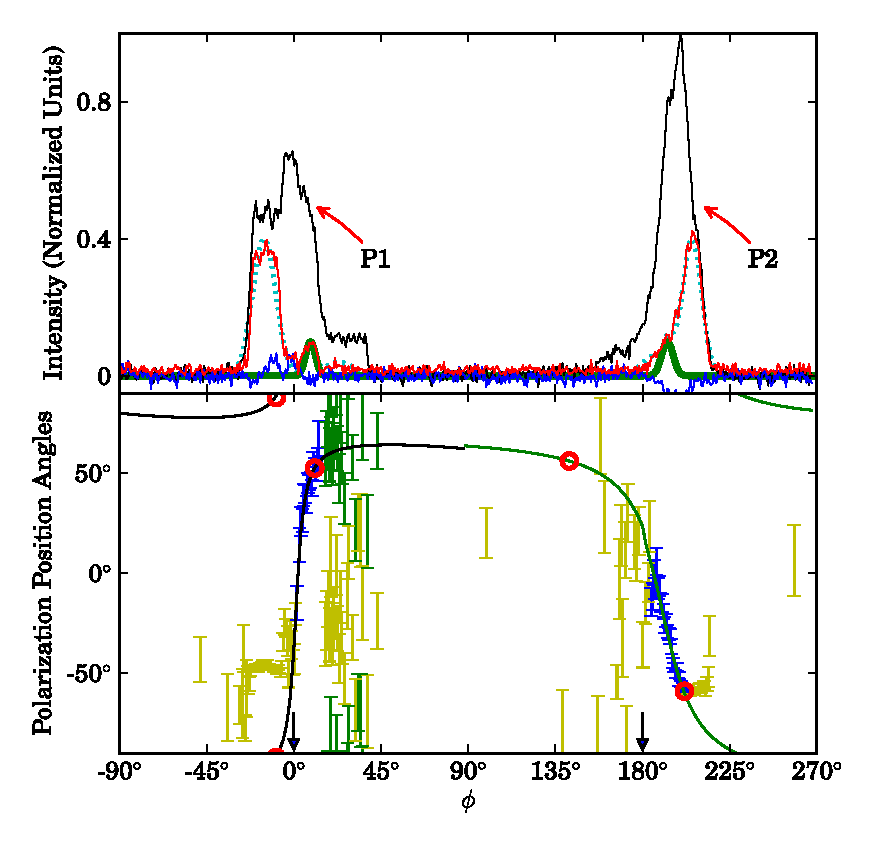
\includegraphics[width=0.9\textwidth]{chapters/multiWaveLength/figures/figure3-0737.eps}
\caption[Polarimetric profile for PSR J$0737-3039$A as observed at 1.4 GHz
with the Parkes radio telescope]{
Figure taken from \cite{guillemot2013fermi}.
Polarimetric profile for PSR J$0737-3039$A as observed at 1.4 GHz
with the Parkes radio telescope (R.~N.~Manchester, private communication). Top panel:
Stokes parameter curves (black is total intensity, red is linear polarized intensity, and
blue is circularly polarized intensity) and Gaussian decomposition
of the linear intensity components (dotted curve is all linear and the thick green
curve gives the rapid sweep central component fit here). Bottom: position angle
data (blue: central components, yellow: other position angle values, green: P1 tail with
an orthogonal mode jump). The smooth curves give the best fit model for the two
poles while the red circles denote the boundaries of the open zone at the
emission altitude. Arrows denote the phase of the closest approach of the
magnetic axes to the Earth line-of-sight.
\label{fig:polarfit}} \end{center}
\vskip -.3truecm
\end{figure*}


\begin{figure*}[t!!]
\begin{center}
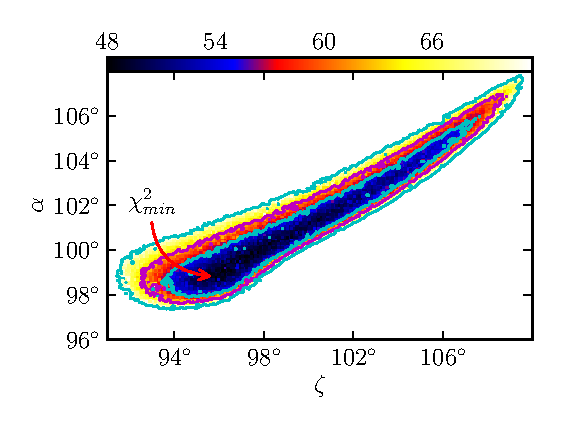
\includegraphics[width=0.9\textwidth]{chapters/multiWaveLength/figures/figure4-0737.eps}
\caption[Map of $\chi^2$ surface of the RVM fit to the radio polarization data
(central components) for PSR J$0737-3039$A in the $\alpha$--$\zeta$
plane]{Figure taken from \cite{guillemot2013fermi}. Map of $\chi^2$
surface of the RVM fit to the radio polarization data (central components) for
PSR J$0737-3039$A in the $\alpha$--$\zeta$ plane. The best fit orientation
angles ($\alpha,\, \zeta$) are indicated by an arrow, while the contours are
shown at the $1\sigma$, $2\sigma$ and $3\sigma$ levels above $\chi^2_{\rm min}$.\label{fig:polarchisq}}
\end{center}
\vskip -.3truecm
\end{figure*}


\begin{figure*}[htbp]
\begin{center}
\includegraphics[width=0.9\textwidth]{chapters/multiWaveLength/figures/figure5-0737.eps}
\caption[Light curves for PSR J$0737-3039$A at the $\alpha$ and $\zeta$ angles determined 
from the radio polarization study]{Figure taken from \cite{guillemot2013fermi}.
Light curves for PSR J$0737-3039$A at the $\alpha$ and $\zeta$ angles determined
from the radio polarization study, and for the outer gap model (solid blue line) and the
two-pole caustic model (dashed green line). The observed radio and $\gamma$-ray profiles are
shown as a solid red line and as a shaded gray histogram, respectively. See
Figure~\ref{fig:polarfit} for the definition of the magnetic axis phase
$\phi_B$. The blue arrow denotes the location of the magnetic axis under the outer gap
and two-pole caustic geometries. \label{fig:lcmodeling2}} \end{center}
\vskip -.3truecm
\end{figure*}


\begin{table*}
\caption{Polarization Fit Parameters for PSR J$0737-3039$A
\label{tab:polarfitpars}}
        \begin{center}{\small
        \def\arraystretch{1.5}
	\begin{tabular}{llllll}
        \hline
$\alpha$ $(^{\circ})$ & $\zeta$ $(^{\circ})$ & $R_{1}/R_{\rm LC}$ & $R_{2}/R_{\rm LC}$ & $\chi^{2}$ & DOF
\\ \hline
${98.8}^{+8}_{-1.5}$ & ${95.8}^{+13.2}_{-4.3}$ & $0.01^{+0.22}_{-0.01}$ & $0.11^{+0.49}_{-0.05}$ & $48$ & $35$
\\ \hline
        \end{tabular}}
\tablecomments{Errors are the extrema of the $1\sigma$ contours in the full
multidimensional parameter space. $R_{1}$ is the emission altitude of the
central component of P1 and $R_{2}$ is the altitude of the central component of
P2.} \end{center}
        \end{table*}




The paper \citep{guillemot2013fermi} reports the detection of 
PSR J0737$-$3039A, the first detection of
a mildly recycled pulsar by the {\it Fermi} Large Area Telescope.  
Such a pulsar is only mildly spun up by its companion.
The pulsar PSR J0737$-$3039A
is in a 2.4 hour orbit with another pulsar
\citep{burgay2003increased,lyne2004double}.
Such a detection is exciting
because it fills in an underpopulated
region of the $P$-$\dot{P}$ picture
\citep{psrcat}.

Further,  understanding the pulsars formation has been 
of interest.
The viewing angle is a measure of the misalignment
between the spin axis and orbital angular momentum
since the inclination of the binary system is 
known.  This measurement in turn is given as $\zeta$
near $90^\circ$ (as discussed below) indicating 
that the misalignment angle is small.
This has important implications on the formation
theory of the system 
\citep{breton2008relativistic,ferdman2013double,podsiadlowski2005double}.

The 1.4 GHz data from Parkes radio telescope was
used in the analysis of 
PSR J0737$-$3039A.
We used orthogonal mode jumps and interstellar
scattering as well as multiple and finite altitude.
We fit only the central components of the two peaks. 
We believed that the trailing edges of
the emission was dominated by plasma effects
and that the present model would not adequately 
capture the field line structure from 
this much higher emission.  Thus we 
favored modeling only the central part
of the polarization of the two radio peaks.
In particular, the flattened components of 
the polarization can not be modeled using
typical magnetic field lines and single altitudes.  
 
Figure~\ref{fig:polarfit} labels the  
Gaussian components used for the intensity 
in the upper panel (green thick line) and the polarization in
the lower panel (blue data points).  
The unmodeled data points are in yellow on
the Figure~\ref{fig:polarfit}.
Trailing edges of $P1$ in linear intensity
are separated from the central component
by linear intensity of zero which suggests
a orthogonal mode jump (for a more in depth 
discussion of this phenomena see Section \ref{sec:MAISOM}). 
The green data points show the
polarization offset by 90$^\circ$.

The black and green solid lines on the lower
panel of Figure~\ref{fig:polarfit} are the best fit model
to the blue polarization data points.
The altitudes for the two components are
different at $0.01R_{\rm{LC}}$ for $P1$ and 
$0.11R_{\rm{LC}}$ for $P2$.  At these altitudes,
The red circles indicate the open zone 
phase expected.  Interestingly, the polarization
not modeled falls outside of this phase, indicating
that the polarization is from higher altitude emission
or from emission within the formal closed zone and hinting
at reasons for its unusual structure.  Indeed, our model is
then one where the central components are from the center
of a hollow cone of emission where the altitude is relatively low
and the wings are from the higher altitudes of the cone.
Full fit parameters and errors are given in Table \ref{tab:polarfitpars}.
The fit map of $\chi^2$ is given in Figure~\ref{fig:polarchisq}.

The results of the polarization fitting were compared to 
$\gamma$-ray light curve modeling results.  Namely,
the polarization fitting produced a phase of closest approach for 
the surface dipole axis.  Both outer gap and two-pole caustic
models produced acceptable light curves in the region
of best fit in the radio polarization as seen in
Figure~\ref{fig:lcmodeling2}.  But the 
model phase zero ($\phi=0$) of the radio and $\gamma$-ray is offset by
$0.1$.  One possible explanation is the lack of 
plasma effects in the modeling.  
For instance, \cite{kalapotharakos2012gamma}
found that including finite conductivity in
magnetohydrodynamics simulations will cause such
a lag compared to vacuum models.

In addition to polarization modeling,
simultaneous fits in radio and $\gamma$-ray
to the light curves
was also performed resulting in
similar geometric angle constrains.

